%%%%%%%%%%%%%%%%%%%%%%%%%%%%%%%%%%%%%%%%%%%%%%%%%%%%%%%%%%%%%%%%%%%%%%%%%%%%%%%%
\documentclass[11pt]{article}

\usepackage[authoryear]{natbib}
\usepackage[top=2.5cm,bottom=2.5cm,left=2.5cm,right=2.5cm]{geometry}
\usepackage{color}
\usepackage{chemarr}
\usepackage{amssymb}
\usepackage{graphicx}
\usepackage{textcomp} 
\usepackage[gen]{eurosym}
\usepackage{amsmath}
\usepackage[margin=1.5cm]{caption}
\usepackage{amsmath,mathtools}
\usepackage{subcaption}
\usepackage{ulem}
%\setlength{\belowcaptionskip}{-5pt}
%\setlength{\abovecaptionskip}{-8pt}
\usepackage{enumitem}

%\usepackage[autolinebreaks,useliterate]{mcode}
\usepackage[usenames, dvipsnames]{xcolor}
\colorlet{shadecolor}{gray!5}
\usepackage{listings}
\lstset{ 
	language=R,                     % the language of the code
	basicstyle=\scriptsize\ttfamily, 	  % the size of the fonts
	numbers=left,                   % where to put the line-numbers
	numberstyle=\tiny\color{Blue},  % the style that is used for the line-numbers
	stepnumber=1,                   % the step between two line-numbers.
	numbersep=5pt,                  % how far the line-numbers are from the code
	backgroundcolor=\color{shadecolor},  % choose the background color.
	showspaces=false,               % show spaces adding particular underscores
	showstringspaces=false,         % underline spaces within strings
	showtabs=false,                 % show tabs within strings adding particular underscores
	frame=tb,                   	  % adds a frame around the code
	rulecolor=\color{Black},        % if not set, the frame-color may be changed on line-breaks within not-black text (e.g. commens (green here))
	tabsize=2,                      % sets default tabsize to 2 spaces
	captionpos=b,                   % sets the caption-position to bottom
	breaklines=true,                % sets automatic line breaking
	breakatwhitespace=false,        % sets if automatic breaks should only happen at whitespace
	keywordstyle=\color{RoyalBlue}, % keyword style
	commentstyle=\color{OliveGreen},% comment style
	stringstyle=\color{ForestGreen} % string literal style
}

\newcommand{\nrtodo}[1]{{\color{blue} NR: #1}}

%%%%%%%%%%%%%%%%%%%%%%%%%%%%%%%%%%%%%%%%%%%%%%%%%%%%%%%%%%%%%%%%%%%%%%%%%%%%%%%%
\title{\textbf{Comparing BC mixing state from CAMChem to SP2 measurements}}
\author{Yinrui Li}
\date{}


%\maketitle


\begin{document}
	\maketitle
	%%%%%%%%%%%%%%%%%%%%%%%%%%%%%%%%%%%%%%%%%%%%%%%%%%%%%%%%%%%%%%%%%%%%%%%%%%%%%%%%
	
	
	
	\section{SP2 Measurement} 
	
	The SP2 instrument measures BC particles in the diameter range from
	approximately 90 to 400~nm, which is unlikely to represent the total
	ambient number and mass concentrations of BC \citep{Reddington2013}.  In order to compare CAMChem model simulated BC with
	observations, we estimated the mass fraction of modeled BC in the size
	range (90--400~nm) corresponding to SP2 measurement.
	
	\section{Estimating the mean BC core diameter in primary carbon mode and in accumulation mode} 
	
	A 4-mode version of the modal aerosol model (MAM4) is applied in
	CAMChem1.2.2. BC is emitted to the primary carbon mode, and then is
	transferred to the accumulation mode by condensation of
	$\rm{H_2SO_4}$, $\rm{NH_3}$ and $\rm{SOA}$ and by coagulation \citep{Liu2012}. In primary carbon mode, particles consist of externally
	mixed BC and OC, whereas in accumulation mode, particles consist of
	internally mixed BC and non-BC material.
	
	SP2 measures the mass size distribution of the BC particle
	cores over a calibrated volume equivalent diameter (VED) range of
	55--400~nm, and the number-detection efficiency at sea level pressure
	is reported to be one for BC above 90~nm VED \citep{Schwarz2010a}. So following Reddington et al., 2013, we use 90~nm as the
	lower bound here.
	
	Both modes assume lognormal distribution as is shown in
	Table~\ref{tab:mam4_modes}. The geometric standard deviation $\sigma_{\rm g}$ is fixed but geometric mean diameter can
	change according to total mass and total number of aerosol particles
	in that mode.
	
	\begin{table}
		\begin{center}
			\begin{tabular}{c c c}
				\hline  
				MAM4 mode & $\sigma_{\text{g}}$ &  10th and 90th percentiles ($\mu$m)		\\   \hline
				Accumulation  & 1.8  &   0.058--0.27 		\\ \hline
				Primary Carbon   & 1.6  &  0.039--0.13  		\\
				\hline			
			\end{tabular}
		\end{center}
		\caption{\label{tab:ozone} Geometric standard deviations ($\sigma_{\text{g}}$) and dry diameter size ranges for MAM4 mode. The size range values are the 10th and 90th percentiles of the global annual average number distribution for the modes (from simulations presented in \citet{Liu2012}).\label{tab:mam4_modes}}
	\end{table}
	
	
	The mean BC core diameter in accumulation mode is interpreted as:
	\begin{align*}
	d = (d_{\text{mixed}}^3 \times f_{\text{BC}})^\frac{1}{3}, 
	\end{align*}
	where $d$ is the mean diameter of BC core,
	$d_{\text{mixed}}$ is the mean diameter of internally mixed particles
	(\textbf{extracted from model}), and $f_{\text{BC}}$ is the volume
	fraction of BC in accumulation mode. For the following estimation of volume fraction within SP2 measurement size range, we refers to BC particle diameter as its core diameter.
	
	\section{Compute Volume Fraction within size range for a Lognormal Distribution}
	The CDF of lognormal number distribution in the geometric diameter range between $d_{1}$ and
	$d_{2}$ is:
	\begin{align*}
	N(d_{1}, d_{2}) = \frac{1}{\text{ln}\sigma_{\text{g}}\sqrt{2\pi}}\int_{d_{1}}^{d_{2}}e^-\frac{(\text{ln}d - \text{ln}d_{\rm g})^2}{2\text{ln}^2\sigma_{\text{g}}}\text{d}(\text{ln}d),
	\end{align*}
	where $d_{\rm g}$ is mean geometric diameter of BC core (extracted from model, varying temporally and spatially). 
	
	The mean volume is proportional to $V(d_{1}, d_{2})$:
	\begin{align*}
	V(d_{1}, d_{2}) &= \frac{1}{\text{ln}\sigma_{\text{g}}\sqrt{2\pi}}\int_{d_{1}}^{d_{2}}d^3e^-\frac{(\text{ln}d - \text{ln}d_{\rm g})^2}{2\text{ln}^2\sigma_{\text{g}}}\text{d}(\text{ln}d)  \\
	&=\frac{e^{\frac{k^2}{2}\text{ln}^2\sigma_{\rm g}+k\text{ln}d_{\rm g}}}{\text{ln}\sigma_{\text{g}}\sqrt{2\pi}}\int_{d_{1}}^{d_{2}}d^3e^-\frac{(\text{ln}d - \text{ln}d_{\text{gv}})^2}{2\text{ln}^2\sigma_{\text{g}}}\text{d}(\text{ln}d),
	\end{align*}
	where the volume mean diameter is represented as $\text{ln}d_{\text{gv}}
	= \text{ln}d_{\text{g}} + 3\text{ln}\sigma_{\text{g}}$
	
	So BC mass fraction (in the size range between 90--400~nm)
	in a mode is derived as:
	
	\begin{align*}
	F(d_{1}, d_{2}) &= \frac{\frac{1}{\text{ln}\sigma_{\text{g}}\sqrt{2\pi}}\int_{d_{1}}^{d_{2}}d^3e^-\frac{(\text{ln}d - \text{ln}d_{\rm g})^2}{2\text{ln}^2\sigma_{\text{g}}}\text{d}(\text{ln}d)}
	{\frac{1}{\text{ln}\sigma_{\text{g}}\sqrt{2\pi}}\int_{0}^{+\infty}d^3e^-\frac{(\text{ln}d - \text{ln}d_{\rm g})^2}{2\text{ln}^2\sigma_{\text{g}}}\text{d}(\text{ln}d)}  \\
	&=\frac{\frac{e^{\frac{k^2}{2}ln^2\sigma_{\rm g}+k\text{ln}d_{\rm g}}}{\text{ln}\sigma_{\text{g}}\sqrt{2\pi}}\int_{d_{1}}^{d_{2}}e^-\frac{(\text{ln}d - \text{ln}d_{\text{gv}})^2}{2\text{ln}^2\sigma_{\text{g}}}\text{d}(\text{ln}d)}{\frac{e^{\frac{k^2}{2}ln^2\sigma_{\rm g}+k\text{ln}d_{\rm g}}}{\text{ln}\sigma_{\text{g}}\sqrt{2\pi}}\int_{0}^{+\infty}e^-\frac{(\text{ln}d - \text{ln}d_{\text{gv}})^2}{2\text{ln}^2\sigma_{\text{g}}}\text{d}(\text{ln}d)}\\
	&=\frac{1}{\text{ln}\sigma_{\text{g}}\sqrt{2\pi}}\int_{d_{1}}^{d_{2}}e^-\frac{(\text{ln}d - \text{ln}d_{\text{gv}})^2}{2\text{ln}^2\sigma_{\text{g}}}\text{d}(\text{ln}d) \\
	&=\frac{1}{2}[\text{erf}(\frac{\text{ln}d_{2} - \text{ln}d_{\text{gv}}}{\sqrt{2}\text{ln}\sigma_{\rm g}})-\text{erf}(\frac{\text{ln}d_{1} - \text{ln}d_{\text{gv}}}{\sqrt{2}\text{ln}\sigma_{\rm g}})],
	\end{align*}
	
	\[F_{\text{accu}}(d_{1}, d_{2}) + F_{\text{pc}}(d_{1}, d_{2}) \neq 1,\]
	BC mass fraction for primary carbon mode ($F_{\text{pc}}(90~\text{nm}, 400~\text{nm})$) and for accumulation mode ($F_{\text{accu}}(90~\rm nm, 400~\rm nm)$) do not add up to 1.
	
	
	\begin{figure}[!h] 
		\begin{center}
			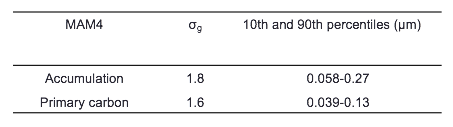
\includegraphics[width = 0.6\textwidth]{Rplot01}
			\caption[]{\label{fig_P1}BC mass mixing ratio ($M_{\rm pc}$ and $M_{\rm accu}$) in primary carbon mode (top) and in accumulation mode (bottom), for surface layer, March.}
		\end{center}
	\end{figure}
	
	\begin{figure}[!h] 
		\begin{center}
			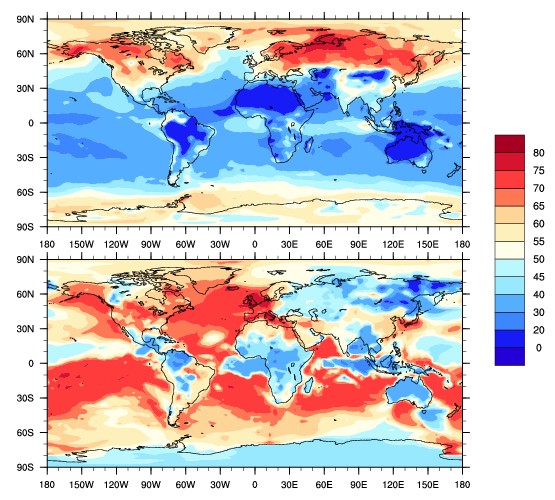
\includegraphics[width = 0.6\textwidth]{Rplot02}
			\caption[]{\label{fig_P2} BC mass fraction between 90 and 400~nm ($F_{\rm pc}$ and $F_{\rm accu}$) in primary carbon mode (top) and in accumulation mode (bottom), for surface layer, March.}
		\end{center}
	\end{figure}
	
	
	\textbf{Within the size range (90--400~nm)}, the ratio of BC mass in each mode to total BC mass is computed as:
	\begin{align*}
	f_{\text{accu}} = \frac{F_{\text{accu}}(d_{1}, d_{2})M_{\text{accu}}}{F_{\text{accu}}(\text{d}_{1}, d_{2})M_{\text{accu}}+F_{\text{pc}}(d_{1}, d_{2})M_{\text{pc}}}\\
	f_{\text{pc}} = \frac{F_{\text{pc}}(d_{1}, d_{2})M_{\text{pc}}}{F_{\text{accu}}(d_{1}, d_{2})M_{\text{accu}}+F_{\text{pc}}(d_{1}, d_{2})M_{\text{pc}}}
	\end{align*}
	\[f_{\text{accu}} + f_{\text{pc}} = 1,\]
	
	where $f_{\text{accu}}$ is the fraction of BC mass in
	accumulation mode, $f_{\text{pc}}$ is the fraction of BC mass in
	primary carbon mode, $M_{\text{accu}}$ and $M_{\text{pc}}$ are BC mass
	in accumulation mode and primary carbon mode, respectively.
	
	Generally, BC mass spreads out more broadly in accumulation mode ($M_{\text{accu}}$) than in primary carbon mode ($M_{\text{pc}}$) (Figure~\ref{fig_P1}). For some Arctic regions, BC in primary carbon mode can be observed higher than BC in accumulation mode, probably due to some local emission sources.
	
	BC mass fraction within SP2 size range ($F_{\text{pc}}(90~\text{nm}, 400~\text{nm})$ and
	$F_{\text{accu}}(90~\rm nm, 400~\rm nm)$) are shown in Figure~\ref{fig_P2}, for primary carbon mode
	(upper panel) and for accumulation mode (lower panel). At the surface,
	SP2 would be able to detect most of BC in primary
	carbon mode at high latitudes ($\textgreater$60$\%$).  At low and
	middle latitudes, this portion is lower than 40$\%$ for most
	regions. SP2 can capture most of BC in accumulation mode when it is
	distant from source regions (e.g., throughout the oceans). We also
	observe that little BC could be seen in either mode for Central
	Africa. \nrtodo{and why is that?} 
	
	$f_{\text{pc}}$ and $f_{\text{accu}}$ are shown in the upper
	and lower panels in Figure~\ref{fig_P3}, respectively. They indicate the mixing state of BC particles
	that can be captured by SP2 measurements. Most of them
	($\textgreater$60$\%$) are internally mixed in low and middle
	latitudes, and are externally mixed in high latitudes. The fraction
	can vary spatially for Arctic region (between 40$\%$ and 70$\%$),
	which should be taken into consideration when comparing modeled BC
	with SP2 measurements. Fractions in two panels should add up to 1.
	
	
	\begin{figure}[!h] 
		\begin{center}
			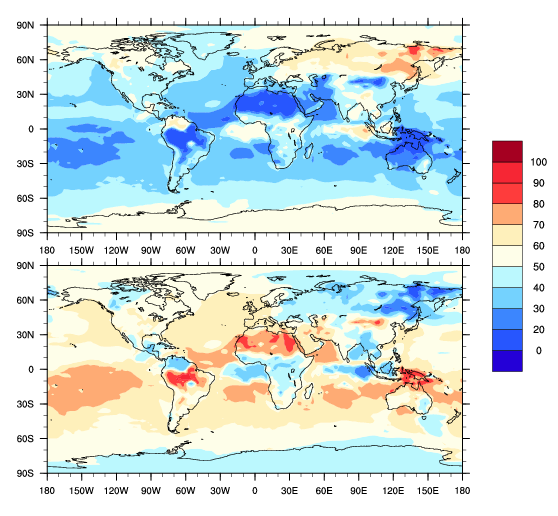
\includegraphics[width = 0.6\textwidth]{Rplot03}
			\caption[]{\label{fig_P3} Ratio of BC mass within SP2 size range to total BC mass within SP2 size range ($f_{\rm pc}$ and $f_{\rm accu}$), in primary carbon mode (top) and accumulation mode (bottom), for surface layer, March.}
		\end{center}
	\end{figure}
	
	
	
	
	
	\clearpage
	
	\bibliographystyle{plain-local-srefid}
	\bibliography{refs}
	
	
	
	
	
	
	%%%%%%%%%%%%%%%%%%%%%%%%%%%%%%%%%%%%%%%%%%%%%%%%%%%%%%%%%%%%%%%%%%%%%%%%%%%%%%%%
	
	
	
\end{document}
%%%%%%%%%%%%%%%%%%%%%%%%%%%%%%%%%%%%%%%%%%%%%%%%%%%%%%%%%%%%%%%%%%%%%%%%%%%%%%%%
%%%%%%%%%%%%%%%%%%%%%%%%%%%%%%%%%%%%%%%%%%%%%%%%%%%%%%%%%%%%%%%%%%%%%%%%%%%%%%%%
